\documentclass[UTF8]{ctexart}
%%%%%%%%%%%%%%%%%%%%%%%%%%%== 引入宏 ==%%%%%%%%%%%%%%%%%%%%%%%%%%%%%
\usepackage{cite}
\usepackage{amsmath}	% 使用数学公式
\usepackage{graphicx}	% 插入图片/PDF/EPS 等图像
\usepackage{subfigure}	% 使用子图像或者子表格
\usepackage{geometry}	% 设置页边距
\usepackage{fancyhdr}	% 设置页眉页脚
\usepackage{setspace}	% 设置行间距
\usepackage{hyperref}	% 让生成的文章目录有链接,点击时会自动跳转到该章节
\usepackage{url}
\usepackage{caption2}

%%%%%%%%%%%%%%%%%%%%%%%%%%== 设置全局环境 ==%%%%%%%%%%%%%%%%%%%%%%%%%%%%
% [geometry] 设置页边距
\geometry{top=2.6cm, bottom=2.6cm, left=2.45cm, right=2.45cm, headsep=0.4cm, foot=1.12cm}
% 设置行间距为 1.5 倍行距
\onehalfspacing
% 设置页眉页脚
\pagestyle{fancy}
%\lhead{左头标}
%\chead{\today}
%\rhead{152xxxxxxxx}
\lfoot{}
\cfoot{\thepage}
\rfoot{}
%\renewcommand{\headrulewidth}{0.4pt}
%\renewcommand{\headwidth}{\textwidth}
%\renewcommand{\footrulewidth}{0pt}

%%%%%%%%%%%%%%%%%%%%%%%%%%== 自定义命令  ==%%%%%%%%%%%%%%%%%%%%%%%%%%%%%%
% 此行使文献引用以上标形式显示
\newcommand{\supercite}[1]{\textsuperscript{\cite{#1}}}
% 此行使section中的图、表、公式编号以A-B的形式显示
\renewcommand{\thetable}{\arabic{section}-\arabic{table}}
\renewcommand{\thefigure}{\arabic{section}-\arabic{figure}}
\renewcommand{\theequation}{\arabic{section}-\arabic{equation}}
% 此行使图注、表注与编号之间的分隔符缺省,默认是冒号:
\renewcommand{\captionlabeldelim}{~}

%===================================== 标题设置  ==========================================
% \heiti \kaishu 为字体设置,ctex 会自动根据操作系统加载字体
\title{\huge{\heiti 基于MPI的相似轨迹计算}}
\author{\small{\kaishu 吉毅}\\[2pt]
\small{\kaishu 苏州大学计算机科学与技术学院}\\[2pt]
\small{Email:}
\url{csyiji@gmail.com}
}
\date{} % 去除默认日期
%\date{\today}

%===================================== 正文区域  ==========================================
\begin{document}
\maketitle
% \tableofcontents % 目录内容,注释取消掉可实现目录

\begin{flushleft}
\textbf{摘要}:利用Open MPI\supercite{openmpi}并行计算环境,实现对于给定轨迹查找与之相似的所有轨迹的实验。\\[8pt]
\textbf{关键词}:并行算法,MPI,相似轨迹,LCSS
\end{flushleft}
\section{实验内容}\label{sec1}

\subsection{背景}
在用户的位置信息和移动轨迹中,蕴含丰富的用户个性信息,对用户移动轨迹研究可有效挖掘用户的行为模式和行为偏好,对智能交通、广告推送、异常轨迹检测、社交推荐等应用有着重要作用。

\subsection{业务场景}
分析移动对象轨迹最常用的应用之一是寻找具有相似轨迹的移动对象并进行归类。一个典型的基于移动对象轨迹的分析场景如下:“对于给定的一个移动对象轨迹,查找与这条轨迹在一定相似度范围内的所有轨迹”。

\subsection{相似度定义}
\label{sec1:subsec3}
最长公共子序列LCSS(Longest Common Subsequence)\supercite{lcss}中对两个 字符串或文本的相似度度量思想:对于两个字符串s1和s2, 尝试找到第三个字符串s3,若s3同时出现在s1与s2中且顺序相同,那么s3 的长度越长则s1与s2越相似。

此处关注的相似度重点在于轨迹经过临近的点、经过各点的顺序两个方面。
点的顺序相同的情况下,经过不同的临近点越多,相似度越高。

\begin{equation}
\label{sec1:subsec3:eq1}
\left\{
\begin{aligned}
& 0 \quad , \quad if \quad A \quad or \quad B \quad is \quad empty. \\
& 1+LCSS_{\delta,\epsilon}(Head(A),Head(B))\quad , \quad if \quad |a_{x,n}-b_{x,m}|<\epsilon \quad and \quad |a_{y,n}-b_{y,m}|<\epsilon \quad and \quad |n-m|\leq \delta \\
& max(LCSS_{\delta,\epsilon}(Head(A),B),LCSS_{\delta,\epsilon}(A,Head(B))) \quad , \quad otherwise
\end{aligned}
\right.
\end{equation}

公式\ref{sec1:subsec3:eq1}是LCSS算法原型公式,其主要分为三点:
\begin{itemize}
	\item 当A或B轨迹中有一个为空,则临近点个数为0;
	\item 否则,循环判断A、B两条轨迹中的各点之间是否满足临近点阈值,是则加1并递归进行;
	\item 否则,将计算的点去掉,分别再与另一轨迹计算是否符合临近点估计,并求两种情况的最大值。
\end{itemize}

利用LCSS可以求出两条轨迹中的临近点个数,然后利用公式\ref{sec1:subsec3:eq2}可计算出轨迹A,B的的相似度。
\begin{equation}
\label{sec1:subsec3:eq2}
\frac{LCSS_{\delta,\epsilon}(A,B)\times2}{m+n}
\end{equation}
\section{重点难点分析}\label{sec2}
\subsection{文件数据的解析}

我们实验的数据由10000个轨迹数据文件和1个索引文件。其整个执行流程如下:

\begin{itemize}
	\item 假设目标轨迹为A,则先根据A的轨迹编号在索引文件中查询,得到行号x与列号y;
	\item 轨迹A数据所在文件名为x\_data ,读取此文件第y行即为轨迹A的内容;
	\item 轨迹的内容结构为:轨迹编号+轨迹数量+轨迹序列..,读取轨迹序列存入二维数组,再进行后续处理。
\end{itemize}

\subsection{LCSS算法阈值选择}

由LCSS算法\ref{sec1:subsec3:eq2}的定义说明,其中计算的判断条件在于轨迹点距离$\epsilon$和轨迹点顺序差$\delta$两个阈值的选择。
而此两个阈值不能仅仅设为常数,它们会随着目标轨迹的变化而变化。因此:

\begin{itemize}
	\item $\epsilon$:选取轨迹上每两个相邻点间的欧式距离和的$\frac{1}{k}$
	\item $\delta$:选取轨迹上点数目的$\frac{1}{k}$
\end{itemize}

\subsection{相似度算法的非递归方式实现}
\label{sec2:subsec3}

\begin{figure}[!htbp]
  \centering
  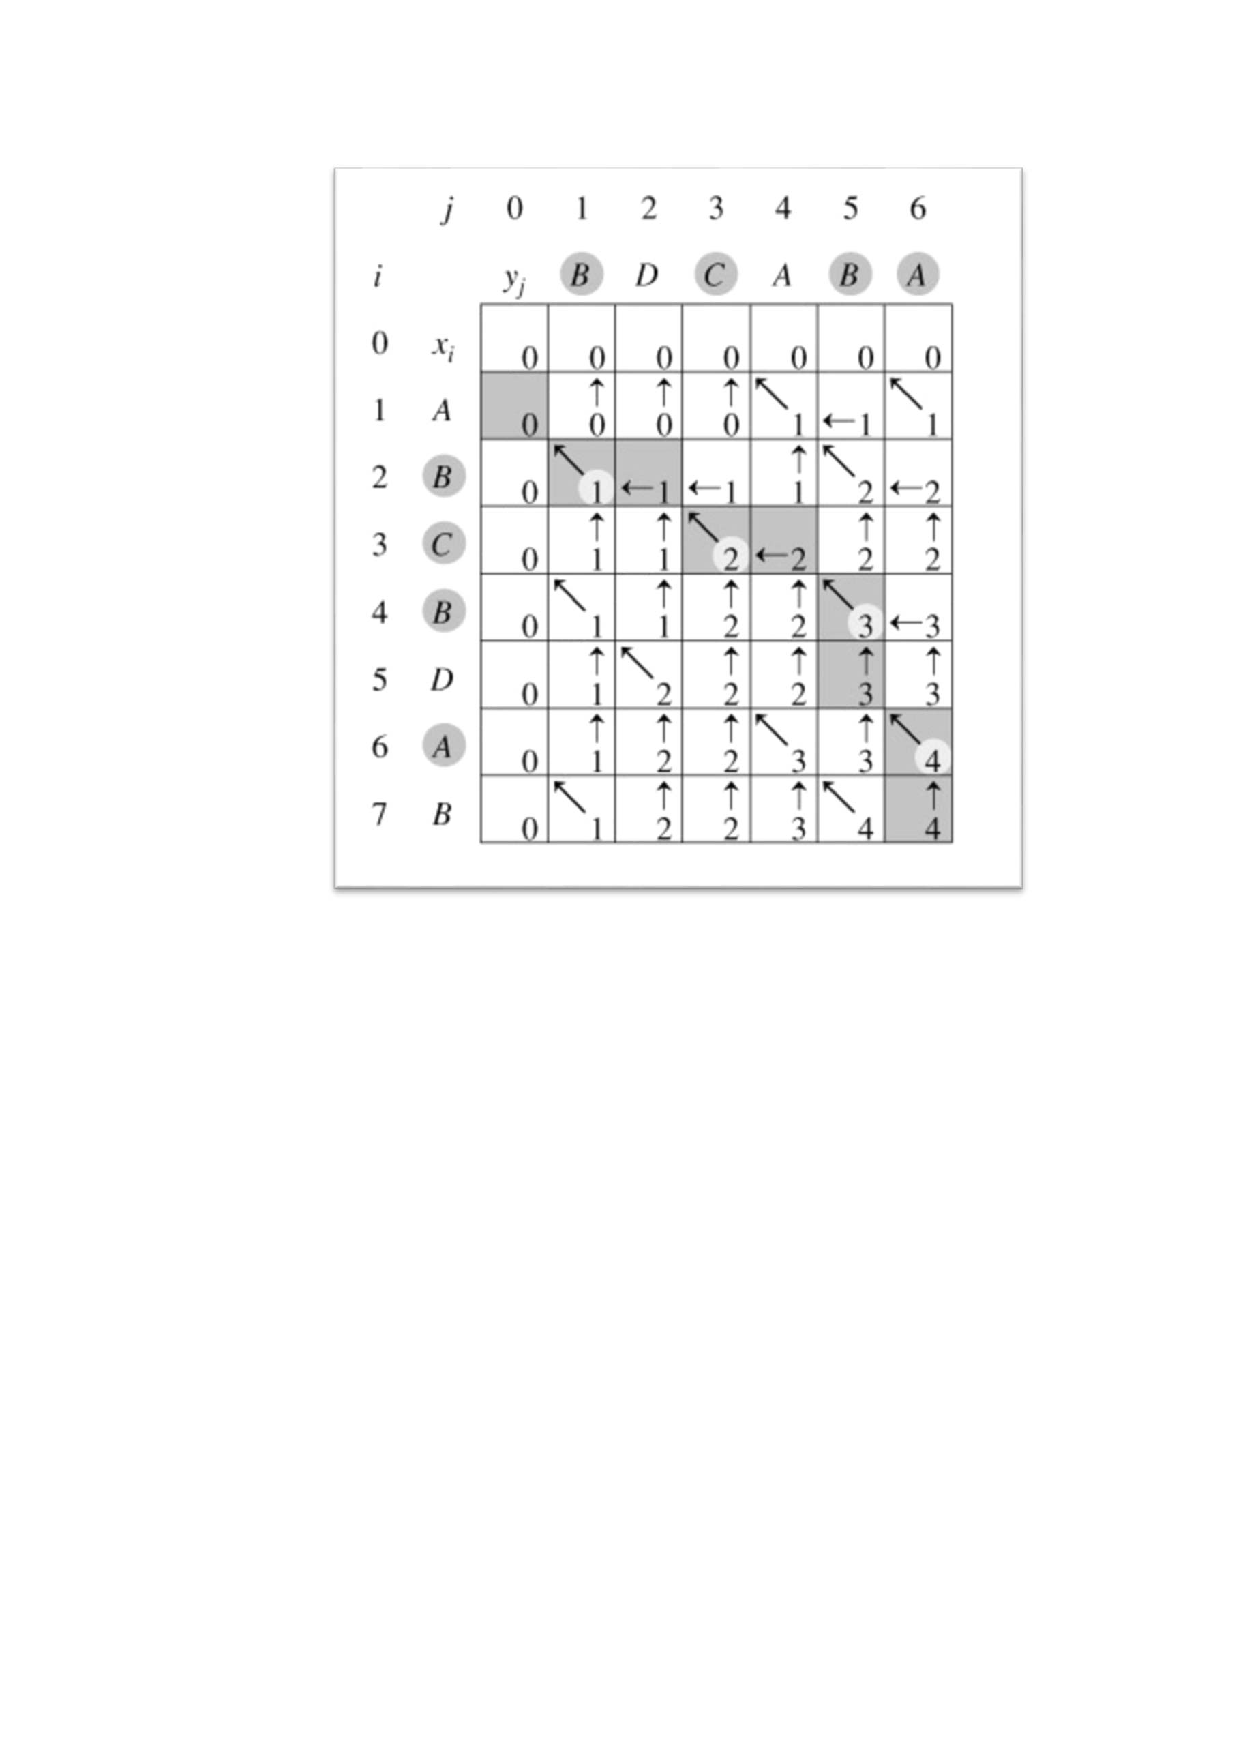
\includegraphics[width=0.35\textwidth]{fig/fig01.pdf}\\
  \caption{LCSS非递归实现}
  \label{sec2:subsec3:fg1}
\end{figure}

LCSS公式\ref{sec1:subsec3:eq1} 给出的是求临近点的递归实现的方式,而我们的每条轨迹点约有60~100个点,则任意两条轨迹计算的递归深度至少为3600,占用的栈空间很大,
因此我们采用非递归方式实现求临近点个数的算法。图\ref{sec2:subsec3:fg1}展示了非递归的实现方式:

\begin{itemize}
	\item 用矩阵来存储任意两点的计算结果,计算主要遵循两个原则:
	\item 轨迹上两点若满足公式里的阈值范围,则将矩阵左上角数值加1;
	\item 轨迹上两点若不满足阈值范围,则选择当前矩阵点的上方和左方的最大的数值作为当前值。
\end{itemize}

\section{计算的技术路线}\label{sec3}
\subsection{文件数据载入}
实验的所有数据都存在文件中,我们共有10000个轨迹数据文件,每个轨迹数据文件中约有1000条轨迹数据,每条轨迹数据约有60-100个点。寻找轨迹的相似轨迹,同一时间我们只关心两条轨迹的数据,因此:

\begin{itemize}
	\item 在加载目标轨迹时,是先从索引文件中读取到轨迹标号的行列,然后读取行对于的数据文件名,加载目标轨迹数据到内存。
	\item 在加载当前对比轨迹时,则直接从数据文件中读取轨迹数据,与目标轨迹进行对比计算。
	\item 并行计算时,在每个进程里都进行以上两个操作,不采用由主进程分发形式。
\end{itemize}

\subsection{计算区域的选择}
\label{sec3:subsec2}
我们的实验数据太多,以至于单进程要跑完所有文件数据将耗费大量的时间,我们的MPI测试环境也对我们的测试进程进行了资源限制。

\begin{figure}[!htbp]
  \centering
  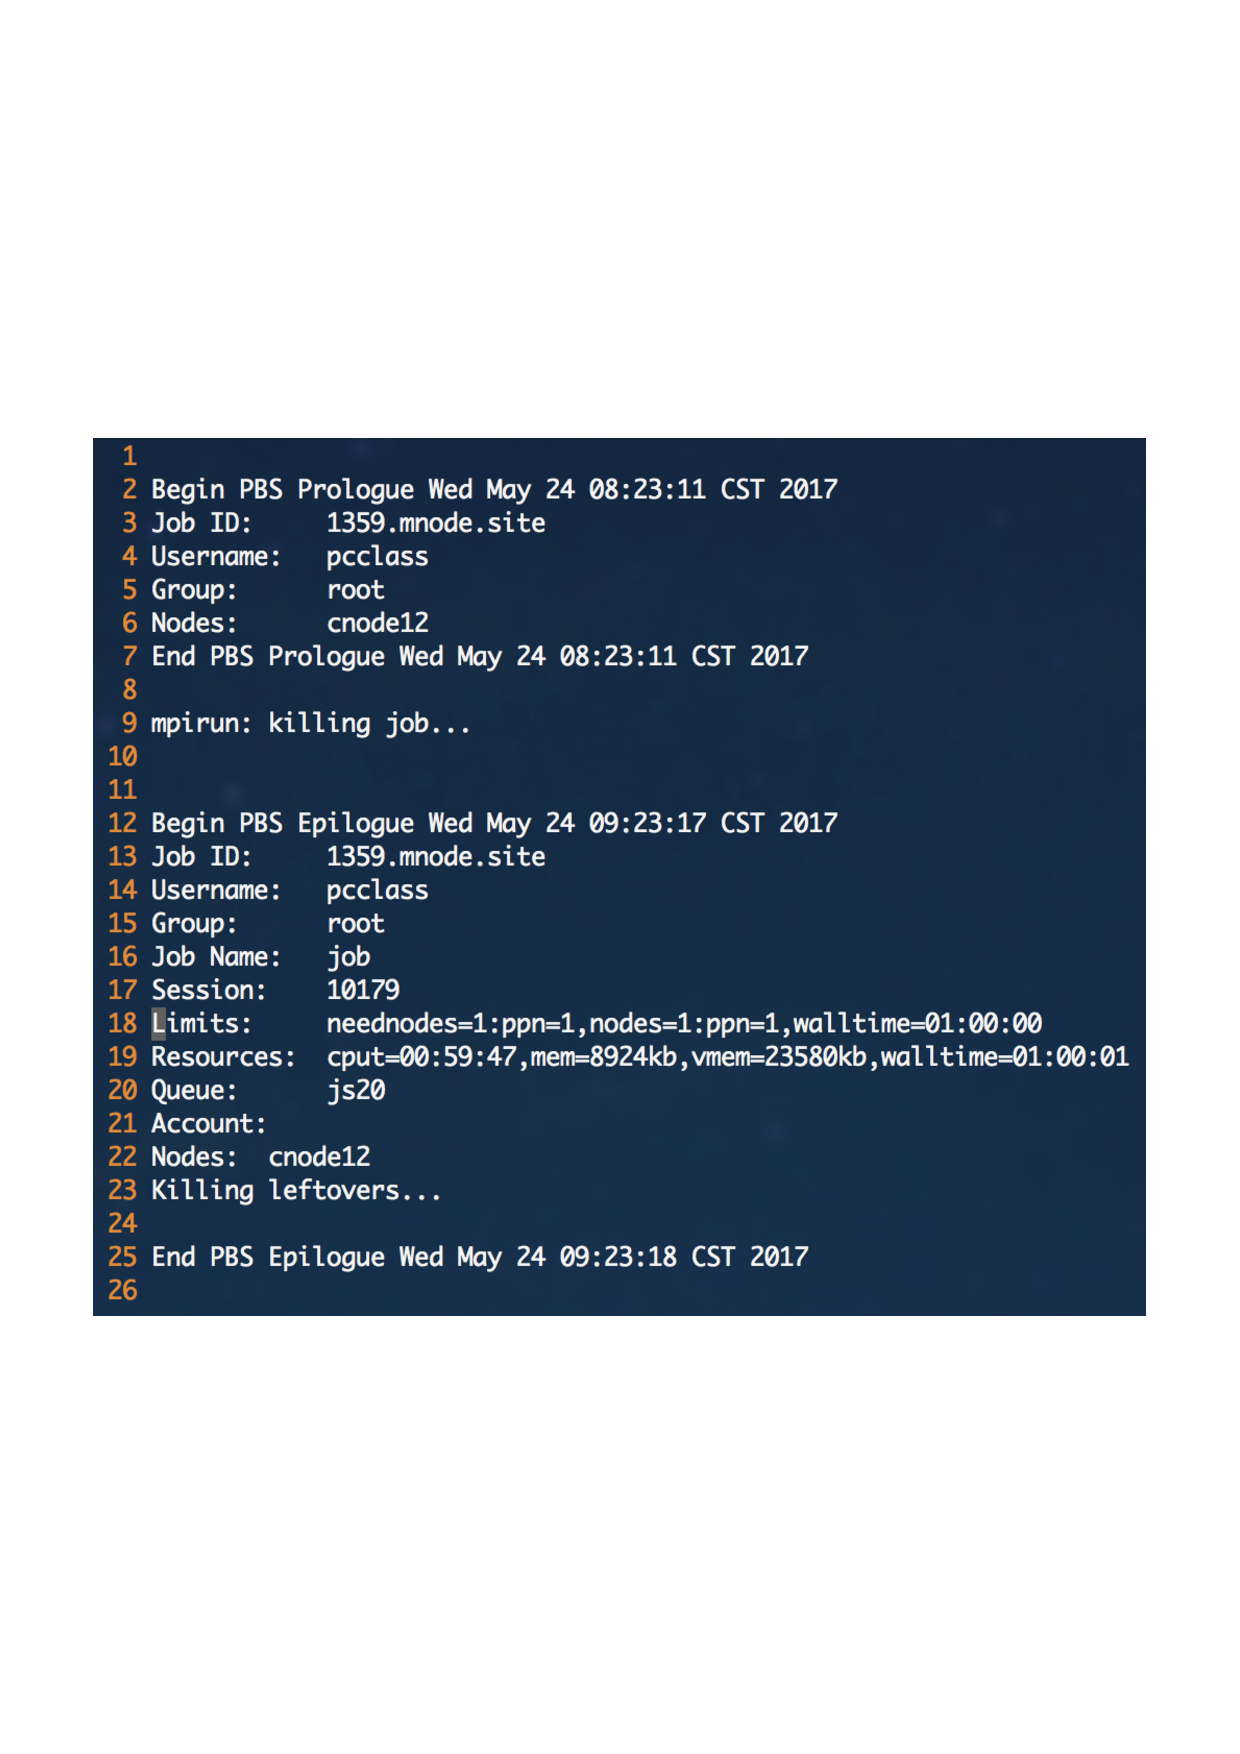
\includegraphics[width=0.5\textwidth]{fig/fig02.pdf}\\
  \caption{MPI测试环境的资源限制}
  \label{sec3:subsec2:fg1}
\end{figure}

如图\ref{sec3:subsec2:fg1}
第18行,显示整个实验环境时间限制在3600秒,超过这个阈值,则会出现第9行所示的结果,我们的任务将被杀死。因此我们进行了一些测试,如表\ref{sec3:subsec2:tb1}所示。

\begin{table}[!htbp]
  \centering
  \caption{基本测试数据}\label{sec3:subsec2:tb1}
  \begin{tabular}{c|c|c}
    \hline
    % after \\: \hline or \cline{col1-col2} \cline{col3-col4} ...
    文件总数量 & 进程总数量  & 所用总时间(秒) \\
    \hline
    10000 & 20 & 2740 \\
    \hline
    10000 & 1 & $>$3600 \\
    \hline
    4 & 4 & 6.56 \\
    \hline
    2 & 2 & 6.67 \\
    \hline
    1 & 1 & 6.7 \\
    \hline
  \end{tabular}
\end{table}

从中可得出大约一个进行执行1个文件查询需要约7秒钟,为了我们程序可在资源限制下运行成功,我们最多可选择500个文件进行MPI实验,而$\surd500=22.6$
实现的搜索区域选择正方形且边长为奇数最简洁,因此我们选择了$21\times21$的矩形区域作为我们的实验目标区域。所有文件名排列矩阵如图\ref{sec3:subsec2:fg2},目标轨迹所在区域的三种情况如图\ref{sec3:subsec2:fg3}。

\begin{figure}[!htbp]
  \begin{minipage}[t]{0.5\linewidth}
    \centering
    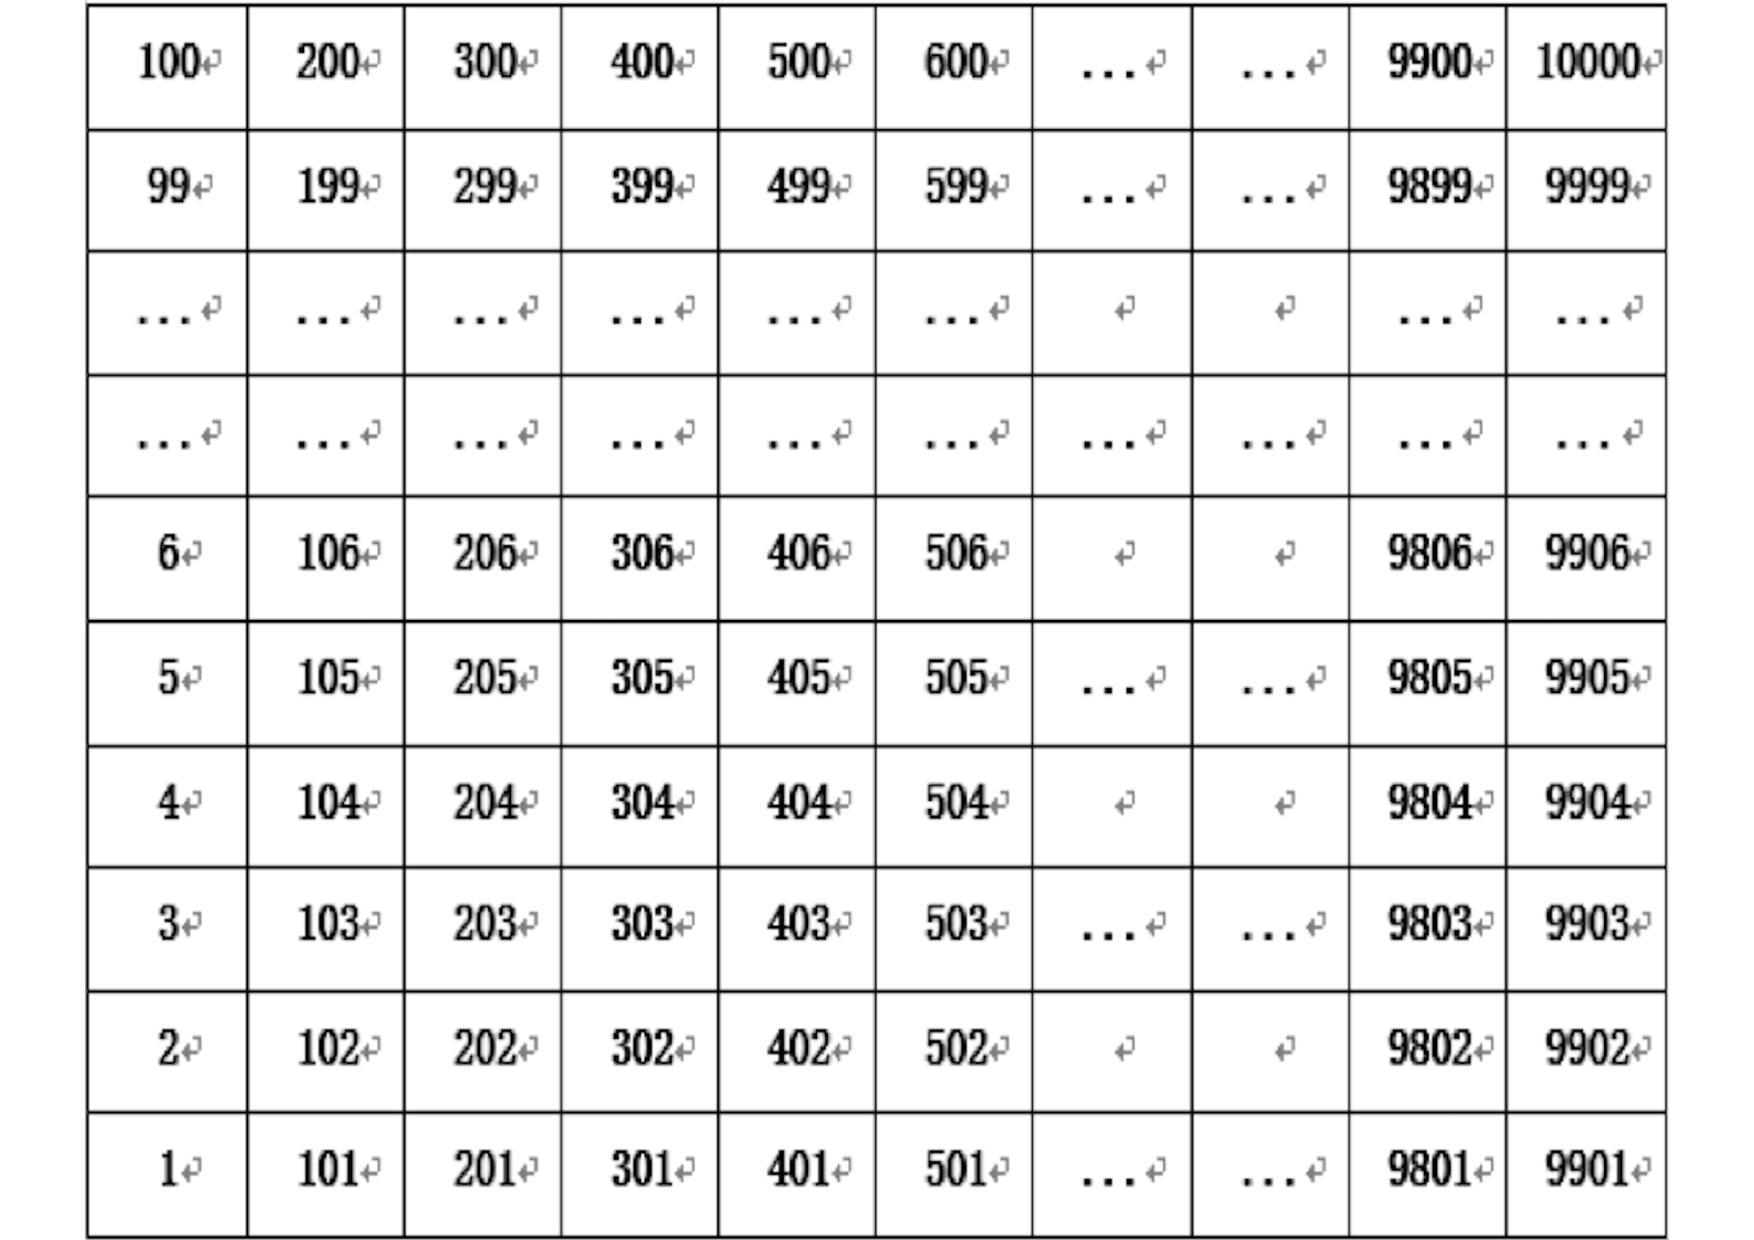
\includegraphics[width=\textwidth]{fig/fig03.pdf}
    \caption{所有文件排列矩阵 \label{sec3:subsec2:fg2}}
  \end{minipage}
  \hfill
  \begin{minipage}[t]{0.45\linewidth}
    \centering
    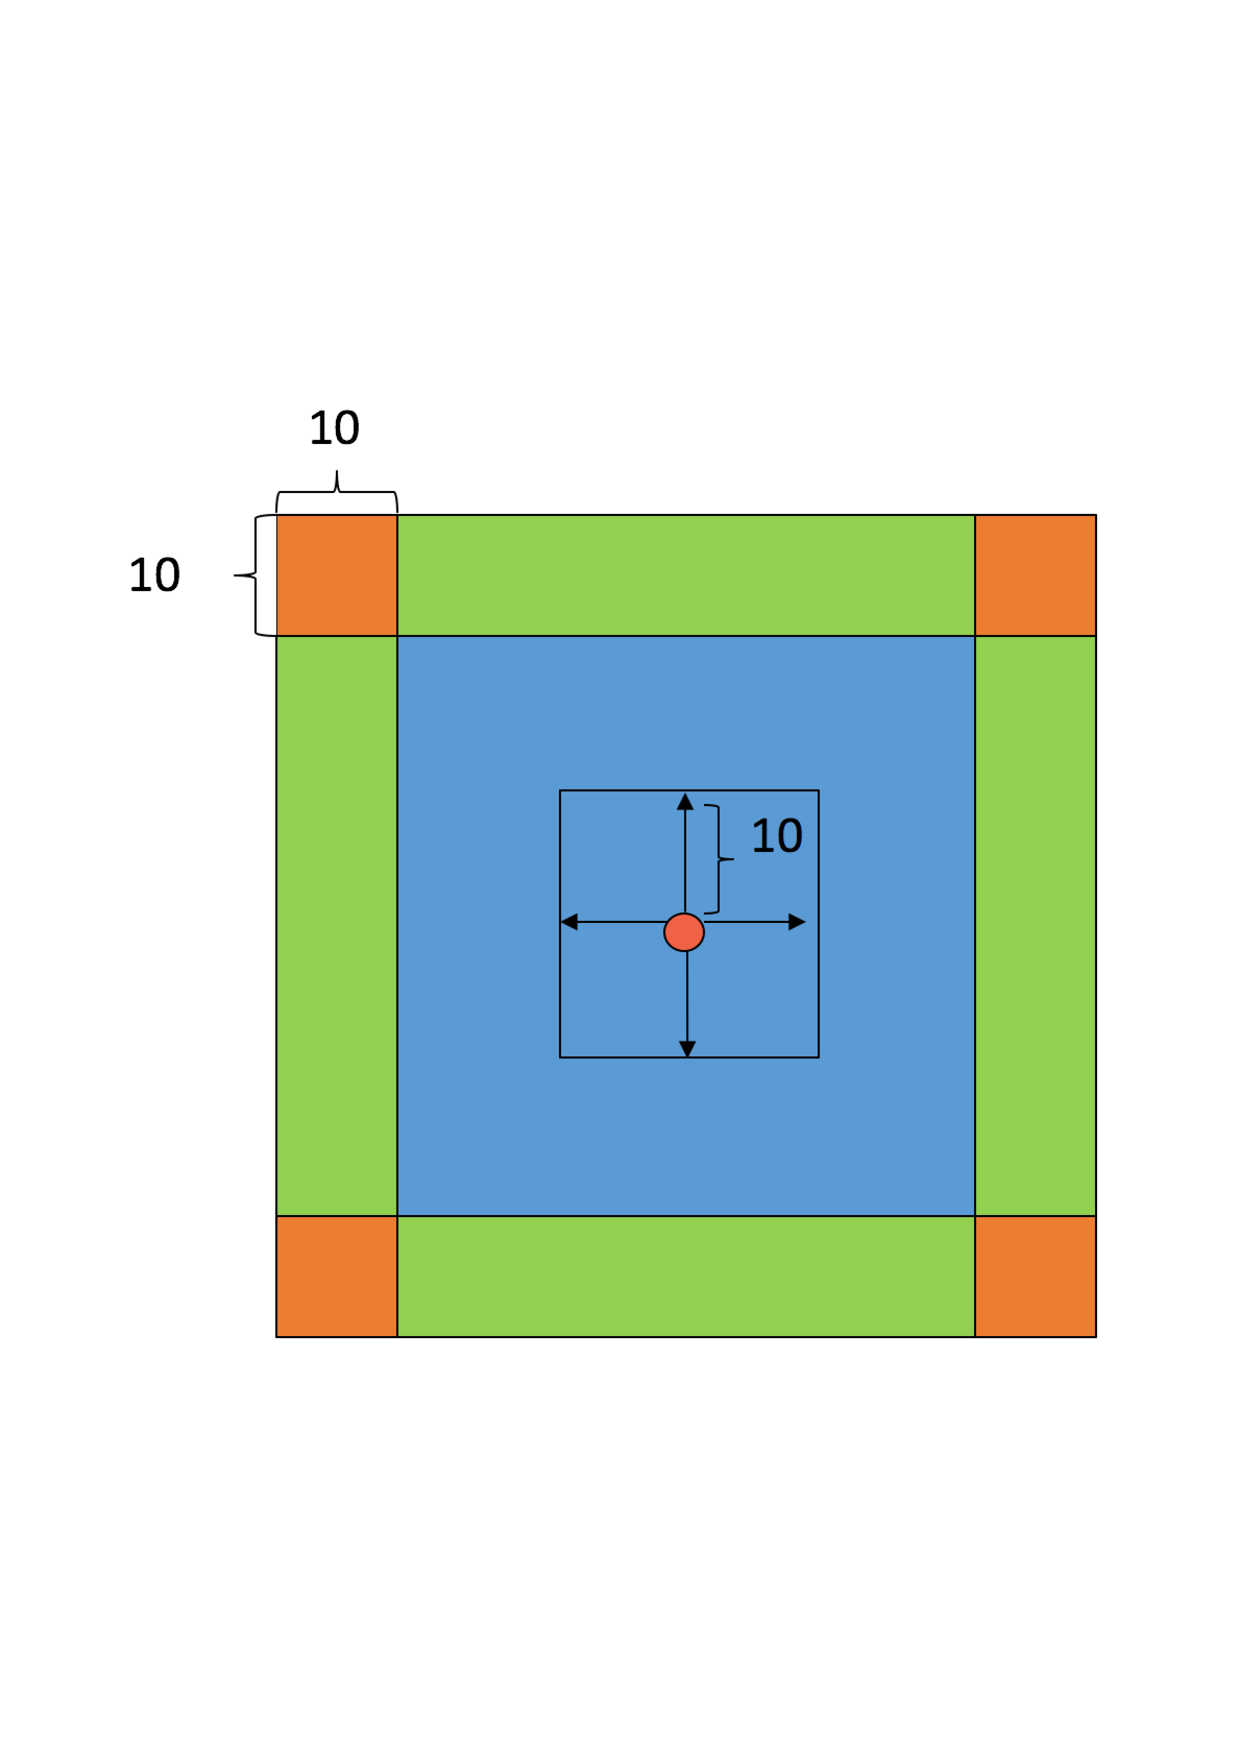
\includegraphics[width=\textwidth]{fig/fig04.pdf}
    \caption{目标搜索区域的三块区域 \label{sec3:subsec2:fg3}}
  \end{minipage}
\end{figure}


\subsection{分片方式}

分片方式采用均分形式,我们在确定了目标搜索区域后,会将$21\times21$的矩阵存到一维数组中,将进程总数量作为递增间隔,每个进程相应地处理各自的一个文件名为等差数列的文件组。

\subsection{通信内容}

在各个进程处理完自己对应的文件组后,会获取到相似轨迹的轨迹编号数组,以0号进程作为主进程,其他进程将计算得到的轨迹编号组发送到0号进程进行汇总。
主要用到MPI并行环境中的MPI\_Send和MPI\_Recv接口。

\section{实验结果及分析}\label{sec4}

\subsection{实验设置}

\begin{itemize}
	\item MPI环境设置:$source /public/home/pcclass/openmpi.sh$
	\item 传入测试数据(10000个数据文件和1个索引文件):$/public/home/pcclass/20164227019/track/cluster$。
	\item 实现MPI接口的C语言源程序:$/public/home/pcclass/20164227019/lcsstrack.c$
\end{itemize}

\subsection{实验步骤}
\label{sec4:subsec2}

\begin{itemize}
	\item 切换到实验目录:$cd \quad /public/home/pcclass/20164227019/$
	\item 编译基于MPI接口的C语言源程序:$mpicc \quad lcsstrack.c$,生成$a.out$可执行文件
	\item 主机测试:$mpirun \quad -np \quad 4 \quad ./a.out$,数字$4$可更改为1-4中的任意数字,表示进程数量。
	\item 多核服务器运行:$qsub \quad hello.pbs$,这里的hello.pbs里默认配置了10个进程进程计算
	\item 自定义进程数运行:$vi \quad hello.pbs$,修改$node2=5:ppn=2$中的数字$5$,$2$和最后一行的$./a.out$前的数字$10$,保证前两数相乘等于最后一个数。则最后一个数据即为实际运行的进程数。
	\item $test01$和$test02$两个文件目录,已经配置好了此实验的各个进程配置文件,$hello.pbs$中后缀即为所配置的进程数量,用户只需$qsub hellox.pbs$即可用相应进程进程测试,最终会在$job$文件中得到结果,结果形式如图\ref{sec4:subsec2:fg1}。
\end{itemize}

\begin{figure}[!htbp]
  \centering
  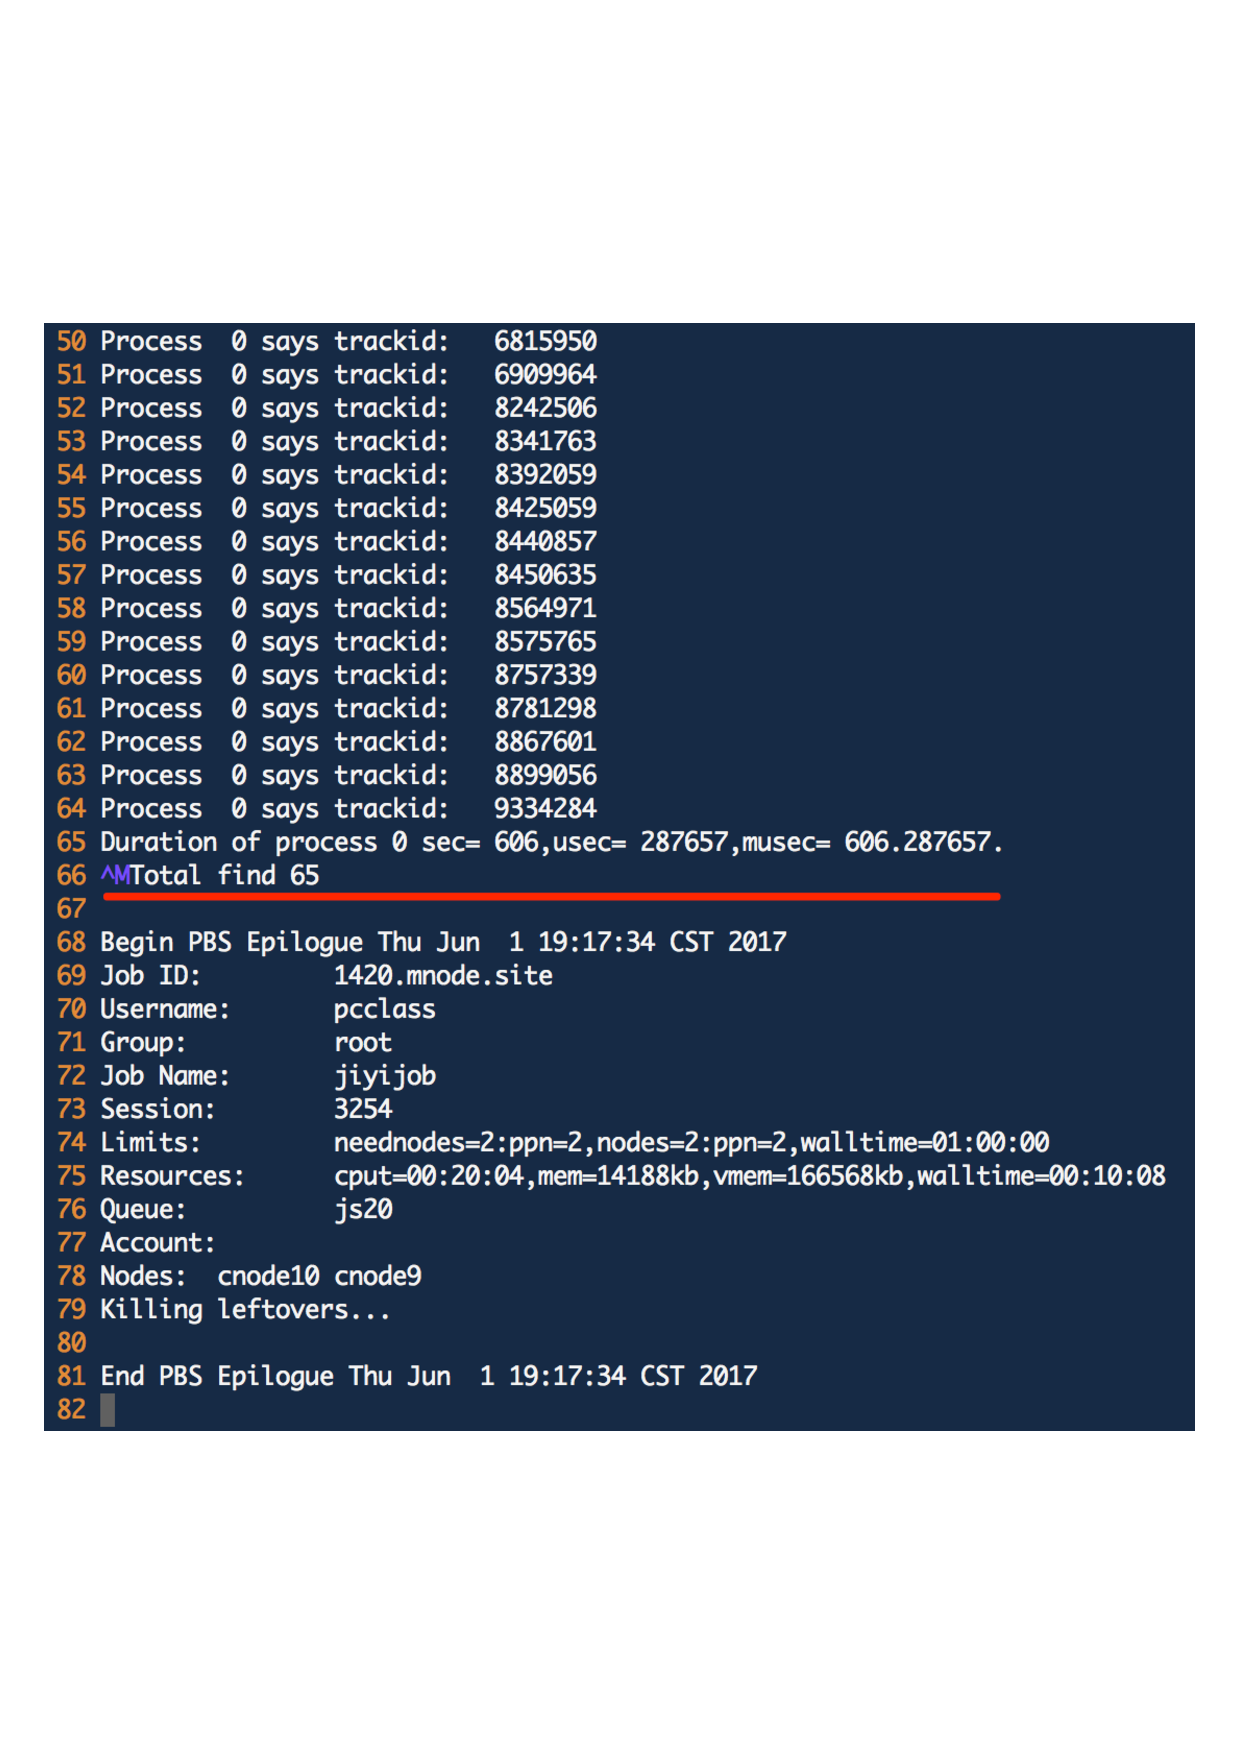
\includegraphics[width=0.55\textwidth]{fig/fig05.pdf}\\
  \caption{实验结果形式}
  \label{sec4:subsec2:fg1}
\end{figure}

\subsection{实验结果}
\label{sec4:subsec3}

我们测试两种形式的结果,一种是轨迹阈值很小时,多个进程间通信数量较少的情况下如表;另一种是轨迹阈值相对较大时,各个进程间通信数量相对较多的情况如表。得到的加速比结果近似于17。

\begin{table}[!htbp]
  \caption{实验结果数据}  
  \centering
  \subtable[通信数量较少]{
  \begin{tabular}{|c|c|c|}
    \hline
    % after \\: \hline or \cline{col1-col2} \cline{col3-col4} ...
    进程总数量 & 时间(秒)  & 比值 \\
    \hline
    1 & 2412 & 1 \\
    \hline
    2 & 1207 & 1.99 \\
    \hline
    4 & 606 & 3.53 \\
    \hline
    6 & 407 & 5.26 \\
    \hline
    8 & 305 & 7.02 \\
    \hline
    10 & 245 & 8.74 \\
    \hline
    12 & 204 & 10.50 \\
    \hline
    14 & 180 & 11.9 \\
    \hline
    16 & 156 & 13.73 \\
    \hline
    18 & 138 & 15.52 \\
    \hline
    20 & 126 & 17 \\
    \hline
    \end{tabular}
  }
  \qquad
  \subtable[通信数量较多]{ 
  \begin{tabular}{|c|c|c|}
    \hline
    % after \\: \hline or \cline{col1-col2} \cline{col3-col4} ...
    进程总数量 & 时间(秒)  & 比值 \\
    \hline
    1 & 2734 & 1 \\
    \hline
    2 & 1369 & 1.99 \\
    \hline
    4 & 689 & 3.96 \\
    \hline
    6 & 459 & 5.95 \\
    \hline
    8 & 347 & 7.87 \\
    \hline
    10 & 281 & 9.72 \\
    \hline
    12 & 231 & 11.8 \\
    \hline
    14 & 223 & 12.2 \\
    \hline
    16 & 176 & 15.5 \\
    \hline
    18 & 158 & 17.3 \\
    \hline
    20 & 126 & 17.6 \\
    \hline
    \end{tabular}
} 
\end{table}


\begin{figure}[!htbp]
  \begin{minipage}[t]{0.5\linewidth}
    \centering
    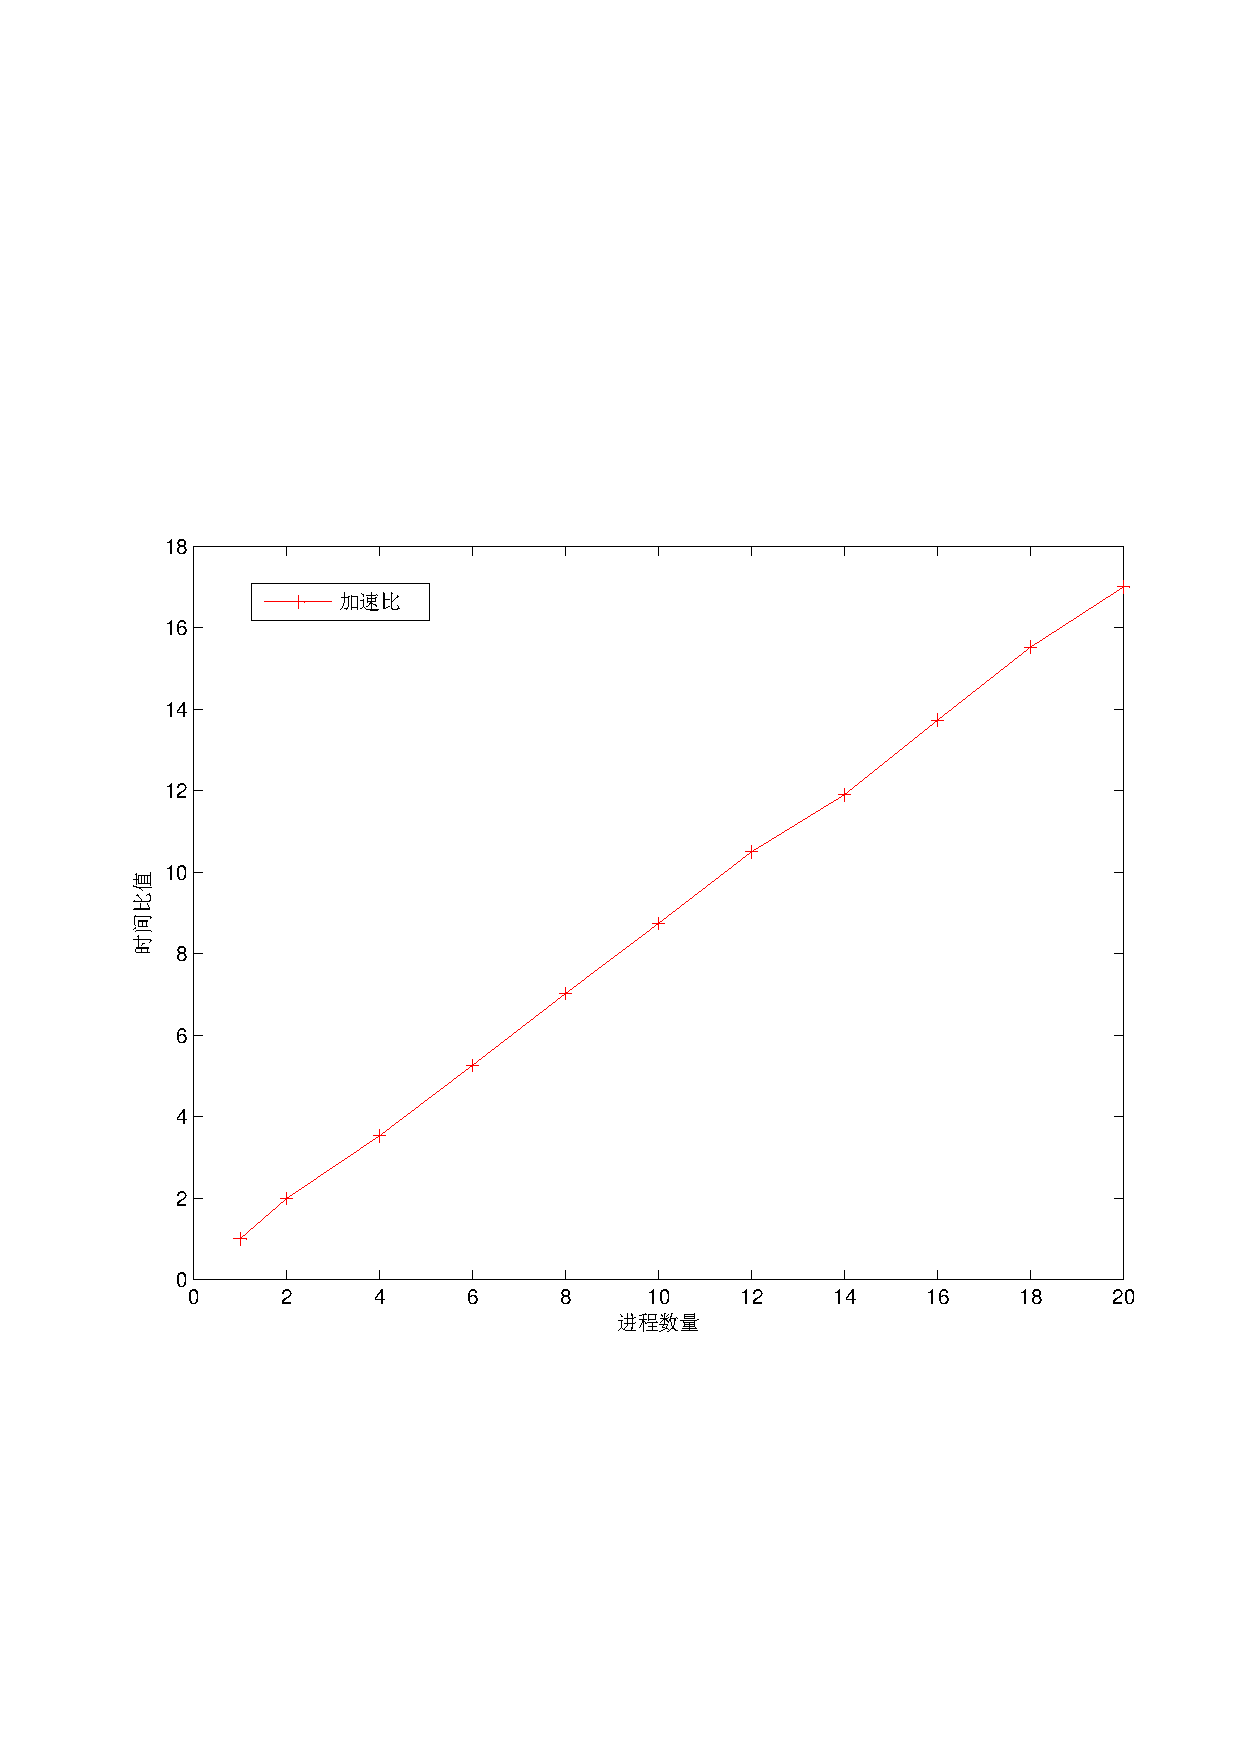
\includegraphics[width=\textwidth]{fig/fig06.pdf}
    \caption{通信较少 \label{sec4:subsec3:fg1}}
  \end{minipage}
  \hfill
  \begin{minipage}[t]{0.5\linewidth}
    \centering
    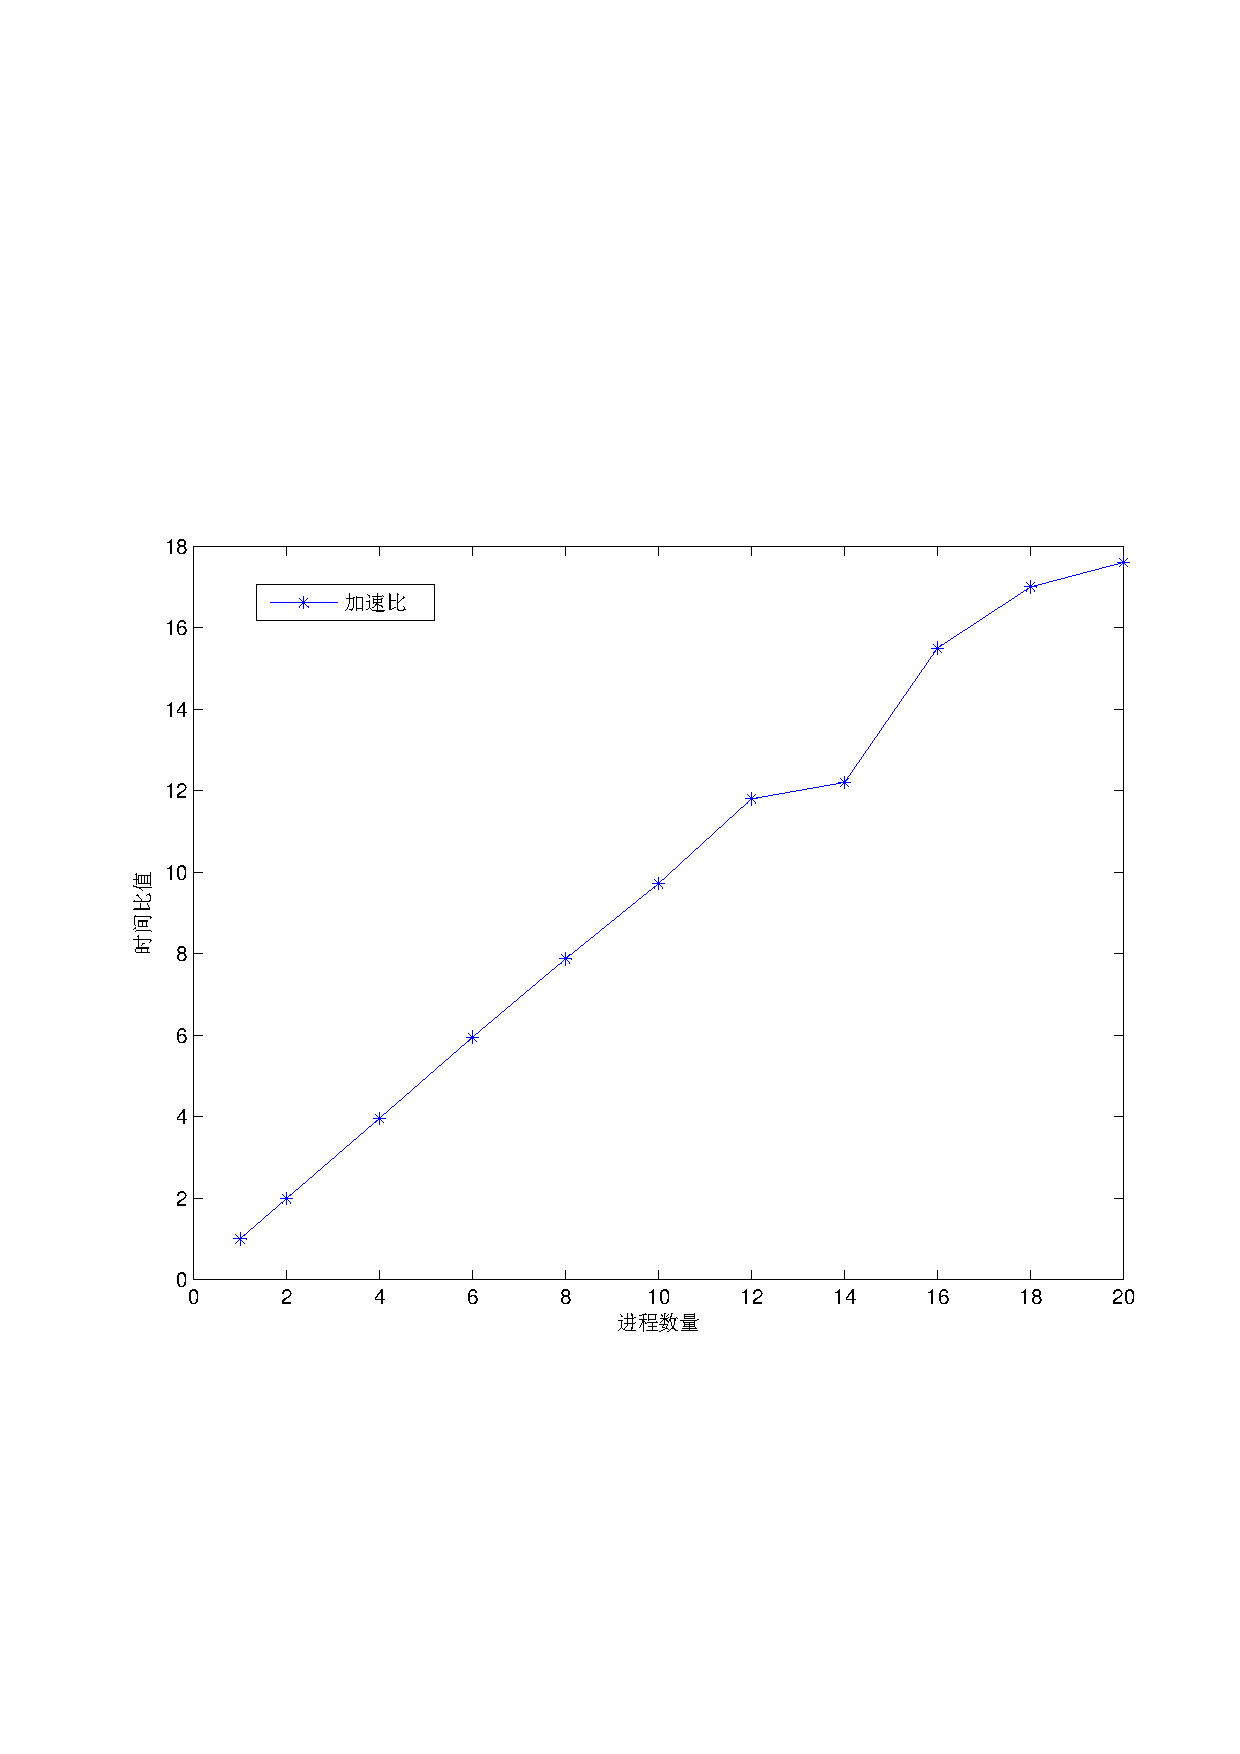
\includegraphics[width=\textwidth]{fig/fig07.pdf}
    \caption{通信较多 \label{sec4:subsec3:fg2}}
  \end{minipage}
\end{figure}

\subsection{实验分析}

由上面的数据可得到此实验的加速比趋近于17,这是一个非常高的结果了。我前后又进行了多次的检查和测试,结果也是基本相同。
主要原因如下
\begin{itemize}
	\item 本实验将文件读取的时间也计算入内了。由于我们的实验数据太多(约13GB),我们不能将所有数据一次性载入内存。因此我们采用的方式是动态载入当前需要对比的轨迹数据。我们的数据文件中每一行都正好是一条轨迹数据,于是我们每读取一条轨迹后就将此轨迹与目标轨迹进行对比,是则记录轨迹编号,否则继续读取下一条数据。
	\item 最后获得相似轨迹的通信数量远远小于计算的轨迹数量,在上面的较多通信的实验中,最终计算得到的相似数据有约13772条,而我们的送计算区域为$441\times1000=441000$条轨迹数据,约是总计算量的$\frac{1}{40}$,通信数量相对较少,导致通信时间几乎忽略不计。我们想将最终获得的数据再调更多,但我们已经将相似度降低到0.2的几乎最低的程度了,几乎达到相似轨迹总量的极限了。
	\item 本实验并行计算方式几乎是独立的,仅在最终结果汇总的时候进行少量的数据通信,相当于规模的平均分配计算,得到的加速比相对较高。
\end{itemize}

\section{提交的文件结构}\label{sec5}
在用pcclass用户名登录实验服务器后,在$20164227019$文件夹中存储的就是我实验所需要的材料:

\begin{itemize}
	\item 实验数据:$track/cluster/$目录下的所有文件。
	\item 源码文件:$lcsstrack.c$ 实现MPI接口的C语言源代码。
	\item MPI环境脚本:$openmpienv.sh$加载MPI库环境。
	\item 并行任务提交脚本:$hello.pbs$里面默认配置了10个进程计算。
	\item 通信较少的实验数据:$test01$里面存储了1个进程和20以内的偶数进程计算的结果。
	\item 通信较多的实验数据:$test02$里面存储了1个进程和20以内的偶数进程计算的结果。
	\item 其他测试数据:$track/test*/$每个test目录下为自己进程实验的其他试验性数据。
\end{itemize}

%===================================== 参考文献  ==========================================
\section{参考文献}\label{sec:sec4}
\bibliographystyle{unsrt}
\bibliography{bib/mpi}

\end{document}